\documentclass[a4paper]{article}
\usepackage[T1]{fontenc}
\usepackage[utf8x]{inputenc}
\usepackage[italian]{babel}

\usepackage{graphicx}
\usepackage{amsmath}
\usepackage{amsthm}
\usepackage{amssymb}
\usepackage{mathtools}
\usepackage{esint}
 \usepackage{import}
\usepackage{xcolor}
\usepackage{geometry}
\geometry{a4paper, top=2cm, bottom=2cm, left=2.5cm, right=2.5cm,  heightrounded, bindingoffset=5mm}


\title{Formulario fisica tecnica}
\author{}
\date{October 2021}

\begin{document}

\newpage
\maketitle
\newpage
\tableofcontents
\newpage	

\newpage 

Novità rispetto al programma;

Al posto degli esercizi sulla trasmissione del calore verranno raccontate alcune esperienze.
Orale: tre domande di teoria (termodinamica, termofluidodinamica, termocinetica o trasporto di massa) Scritto: due esercitazioni, una sulle miscele aria-vapore (studio del benessere ambientale, saper regolare ambienti in ambienti clinici), cicli frigoriferi, terza domanda semi teorica (raccontare una delle esercitazioni citate sopra). 
Esercitazioni sulla criochirurgia, sulla termoregolazione del corpo umano, sul trasporto di massa in aorta aneurismatica, sul trasporto di massa nel circolo di Willis e sull’acustica ovvero rumore provocato dalle valvole stenotiche. Non ci sono esercizi sulla trasmissione del calore e termofluidodinamica.
Testo: Problematiche di fisica tecnica in ingegneria medica (9 capitoli, da Texmat). Risultati di lavori fatti da colleghi o in tesi di dottorato o nella tesi magistrale ecc.
Lezione interrotta causa problemi di connessione. Appello straordinario; chiedere alla segreteria Scritto e orale nello stesso appello.

\newpage 


\section{Termodinamica}
	
\subsection{Introduzione}
	
COMPLETA DA pg 10 


La prima cosa che bisogna fare nella termodinamica classica è definire l’oggetto del nostro studio, cioè l’insieme dei corpi che vogliamo studiare e che chiameremo sistema termodinamico (insieme degli oggetti che vogliamo studiare), si decide quale sistema termodinamico si vuole studiare, ad esempio l’aria nella stanza.
Nel momento in cui decidiamo il sistema, decidiamo anche il contorno fisico del nostro sistema termodinamico S scelto arbitrariamente; quello che c’è all’interno del nostro sistema è l’oggetto del nostro studio, tutto il resto è l’esterno E, mentre S è all’interno del contorno fisico.
Sistema termodinamico   oggetto del nostro studio.
Vogliamo relazionare il sistema termodinamico, cioè quello che c’è all’interno, con l’esterno e in particolare ci interessa la relazione, ovvero le interazioni tra l’interno e l’esterno, cioè ci interessa quello che succede NEL sistema.

COMPLETA 

Definizione fisica del \textbf{lavoro}: si parte dal sistema cilindro-pistone \begin{equation}
	l_i=\int_1^2 p_idv
\end{equation}

\textbf{Convenzione termodinamica}: lavoro positivo se fatto dal sistema verso l'esterno.

\textbf{Convenzione termodinamica}: calore positivo se assorbito dal sistema (convezione opposta al lavoro).
\textbf{Temperatura}:



\subsection{Misure}

Grande intensive --> minuscole
Grandezze intensive --> maiuscole

Misura della pressione 

Il barometro misura la pressione assoluta $p_A=\rho g h$

Manometro differenziale: dislivello => differenza di pressione. Bilancio delle forze : $ \rho S+\rho S\Delta z g=p_AS+\rho_m S\Delta z g$
 
Allora si ottiene che la pressione del fluido in esame rispetto la pressione atmosferica è $\rho -\rho_A=\rho_m \Delta zg$ 

\subsection{Frigoriferi ad effetto termoelettrico}


Permettono di misurare la temperatura. 

\textbf{Effetto Seebeck}

COMPLETA

\textbf{Effetto Peltier} completa


\textbf{Effetto Thompson} 
Corrente in un conduttore metallico $\Longrightarrow$ differenza di temperatura. La quantità di calore che viene scambiata con l’esterno è in valore
assoluto proporzionale alla corrente, alla differenza di temperatura e ad un coefficiente che è chiamato coefficiente di Thomson.
$$\left|d \dot{Q}_{T}\right|=|\tau I d T|=\left|\tau I \frac{d T}{d x} d x\right|$$ 

\subsection{Principio zero della termodinamica}
\textbf{Principio zero della termodinamica} o di Fowler. Presi due corpi A in equilibrio con C tramite una parete conduttrice. E il corpo B in equilibrio con lo stesso C. Allora, essendo entrambi in equilibrio con C, saranno A in equilibrio con B. $Longrightarrow$ Possiamo usare C come termoscopio, per misurare se due corpi sono in equilibrio termico. 

\textbf{calore}
È l’interazione tra il sistema termodinamico e l’esterno, che avviene a causa di una differenza di temperatura, attraverso il contorno (tanto all’interno c’è equilibrio e non mi interessa). Questa definizione è generale, c'è anche quella operativa. 

\subsection{Primo principio della termodinamica}
Il primo principio della termodinamica stabilisce che il lavoro scambiato in una trasformazione termodinamica {\color{red}{ciclica}} in un sistema {\color{red}{chiuso}} è uguale al calore totale scambiato: 
\begin{equation}
	L=Q
\end{equation}		
Ricorda Esperienza di Joule e il fatto che lavoro e calore sono sono negativi (lavoro assorbito e calore ceduto) $-|L|=-|Q|$

Generalizzando vale l'uguaglianza integrale e quindi $dQ-dL=dE$ nota come \textbf{energia totale} e si tratta di una funzione di stato infatti $\oint dE=0$.

L'energia totale dipende da variabili interne e variabili esterne. $E=E_{interne}+E_{esterne}$
Tra le variabili esterne troviamo:
\begin{itemize}
	\item velocità del baricentro
	\item quota del baricentro
\end{itemize}
Allora $\Delta E_e=\Delta E_c+\Delta E_p$ (energia cinetica e potenziale).

Tra le variabili interne troviamo:
\begin{itemize}
	\item variabili termodinamiche (pressione, volume specifico, temperatura)
	\item componenti elettrochimiche (reazioni chimiche, fenomeni elettrici o termoelettrici)
\end{itemize}
Allora $\Delta E_i=\Delta u+\Delta u_x$ (energia interna termodinamica e energia interna di origine elettrochimica).

\textbf{Primo principio della termodinamica per un sistema chiuso che compie trasformazioni aperte}: 
\begin{equation}
	Q-L=\Delta u+\Delta E_c +\Delta E_p 
\end{equation}

In termini differenziali:
\begin{equation}
	dq-dl=du+du_x+{dw^2\over 2}+g dz 
\end{equation}

\begin{figure}[h!]
	\begin{center}
		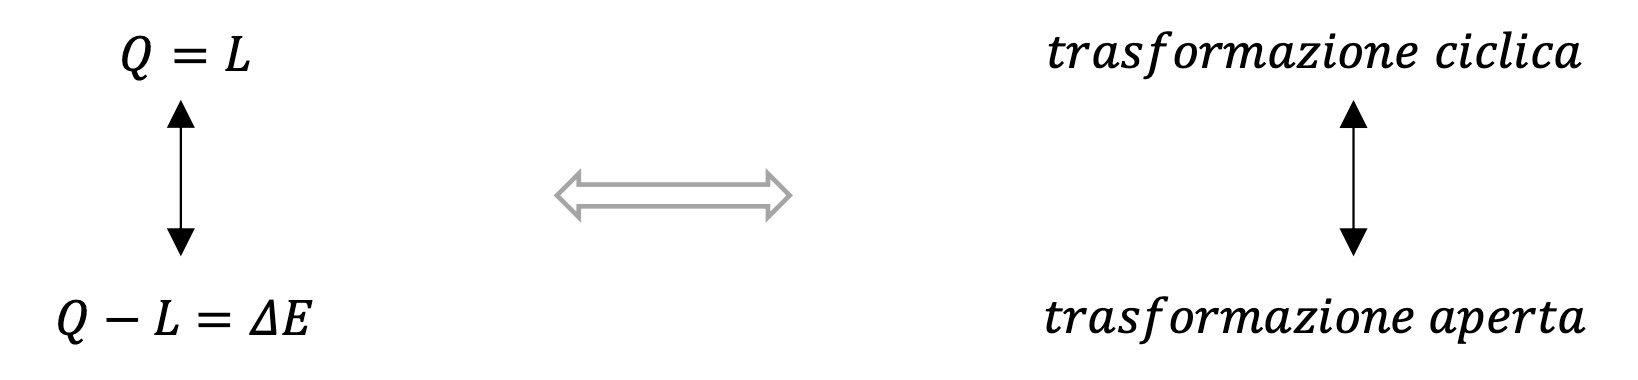
\includegraphics[width=0.6\columnwidth]{generalizprincipio.jpg}
	\end{center}
\end{figure}

\subsection{Calore}
\textbf{Definizione operativa}: il calore si misura come il lavoro scambiato da un sistema in un'esperienza di Joule. Ovvero un sistema chiuso che compie una trasformazione ciclica. 






\newpage
\section{Tesine}

\end{document}